\documentclass{ximera}
\newcommand{\RR}{\mathbb R}
\renewcommand{\d}{\,d}
\newcommand{\dd}[2][]{\frac{d #1}{d #2}}
\renewcommand{\l}{\ell}
\newcommand{\ddx}{\frac{d}{dx}}
\newcommand{\dfn}{\textbf}
\newcommand{\eval}[1]{\bigg[ #1 \bigg]}

\author{Bart Snapp\and Nela Lakos}
\license{Creative Commons 3.0 By-NC}
\acknowledgement{https://www.whitman.edu/mathematics/calculus/}
  \outcome{Interpret an optimization problem as the procedure used to make a system or design as effective or functional as possible.}
  \outcome{Set up an optimization problem by identifying the objective function and appropriate constraints.}
  \outcome{Solve optimization problems by finding the appropriate absolute extremum.}
  \outcome{Solve basic word problems involving maxima or minima.}
\begin{document}
\begin{exercise}

  
  A box with square base and no top is to hold a volume $100$.  Find
  the dimensions of the box that requires the least material for the
  five sides.
  \begin{hint}
  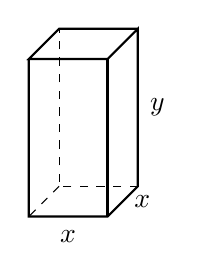
\begin{tikzpicture}

\pgfmathsetmacro{\xr}{2}
\pgfmathsetmacro{\xl}{1}
\pgfmathsetmacro{\yt}{0}
\pgfmathsetmacro{\yb}{-2}
\pgfmathsetmacro{\zi}{0}
\pgfmathsetmacro{\zo}{1}
  \draw[thick](\xr,\yt,0)--(\xl,\yt,\zi)--(\xl,\yt,\zo)--(\xr,\yt,\zo)--(\xr,\yt,\zi)--(\xr,\yb,\zi)--(\xr,\yb,\zo)--(\xl,\yb,\zo)--(\xl,\yt,\zo);
  \draw[thick](\xr,\yt,\zo)--(\xr,\yb,\zo);
  \draw[dashed](\xr,\yb,\zi)--(\xl,\yb,\zi)--(\xl,\yt,\zi);
  \draw[dashed](\xl,\yb,\zi)--(\xl,\yb,\zo);
  \draw(\xr+.25,\yt*.5+\yb*.5,\zi) node{$y$};
  \draw(\xr+.25,\yb,\zi*.5+\zo*.5) node{$x$};
  \draw(\xl*.5+\xr*.5,\yb-.25,\zo) node{$x$};

  \end{tikzpicture}
  \end{hint}
  \begin{hint}
  The dimensions that will result in  "least material" for the five sides are dimensions that result in "smallest surface area".
  So, the quantity that we have to "minimize" is the surface area, $S$.
  \end{hint}
  \begin{hint}
  We have to "minimize"  the surface area, $S$.
  
  $S=x^2 +4xy$
  
  Remember, no top!
  \end{hint}
    \begin{hint}
Next, we express $S$ as a function of, say, $x$.
In order to do that, we have to express $y$ in terms of $x$.


We know that  $V=100$. Therefore,

$x^2\cdot \answer{ y}=100$,
and 

$y=\frac{100}{\answer{x^2}}$.
  
 It follows that 
  
   $S(x)=x^2 +\frac{400}{\answer{x}}$.

  \end{hint}
  \begin{hint}
  So, we have to find the (global) minimum of $S$ on its domain, $(0,\answer{\infty})$.
  We have to find critical points of $S$.
  Therefore, we have to compute $S'(x)$.
  \end{hint}
  \begin{hint}
  $S'(x)=2x-\frac{400}{\answer{x^2}}$.
    \end{hint}
     \begin{hint}
     We have to find critical points of $S$.
     So, we have to solve the equation
     
  $2x-\frac{400}{\answer{x^2}}=0$.
  
  It follows that $S$ has the only critical point  $x=\answer{200^{\frac{1}{3}}}$.
    \end{hint}
  
     \begin{hint}
     Since
    
     $S'(x)=2x-\frac{400}{x^{2}}=\frac{2(x^{3}-200)}{x^{2}}$, it follows that
    
      $S'(x)<0$ on $(0, 200^{\frac{1}{3}})$ and  that $S'(x)>0$ on $(200^{\frac{1}{3}},\infty)$.
     
      This means that $S$ is decreasing on $(0, 200^{\frac{1}{3}})$ and increasing on $(200^{\frac{1}{3}},\infty)$.
      That means that the function $S$ has both a local minimum and global minimum at $x=c$.
 \end{hint}
   


  So, the dimensions that minimize the surface area are
  
  \begin{prompt}
  \[
  \text{width}=\answer{(2) 5^{2/3}},\qquad
  \text{length}=\answer{(2) 5^{2/3}},\qquad
  \text{height}=\answer{5^{2/3}}
  \]
  \end{prompt}
\end{exercise}
\end{document}
